Lastly, this section presents the final Tritium detector, a schematic design of which is shown in the figure \ref{fig:TritiumDetectorSchematicDesign}.

\begin{figure}[h]
\centering
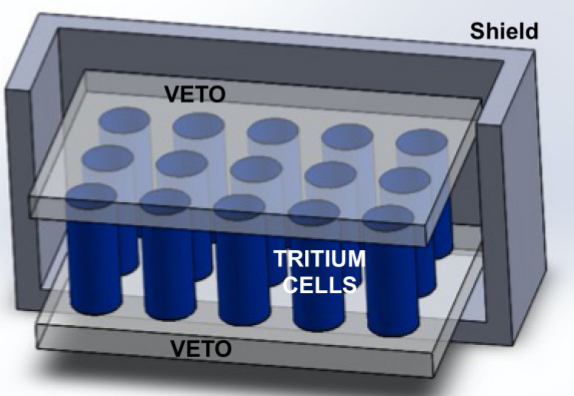
\includegraphics[scale=0.5]{5Prototypes/55ModularTritiumDetector/FinalTritium.png}
\caption{A schematic design of the Tritium detector.\label{fig:TritiumDetectorSchematicDesign}}
\end{figure}

It consists of several Tritium modules, figure \ref{fig:TritiumDetectorSchematicDesign}, which will be read in parallel. Each module will be the prototypes that achieves better results, Tritium-Aveiro 0 (section \ref{subsec:TritiumAveiro}) or Tritium-IFIC 2 (section \ref{subsec:TritiumIFIC2}).

These modules will be isolated from environmental radioactivity using three different techniques.

\begin{enumerate}

\item{} First, an external lead shielding, figure \ref{fig:TritiumDetectorSchematicDesign}, is used to stop the radioactivity coming from the place where the tritium monitor will be located before it reaches the tritium detector.

\item{} Second, several active vetos, figure \ref{fig:TritiumDetectorSchematicDesign}, placed below and above the tritium modules, will be read in anticoincidence to eliminate the effect on the tritium measurement that has the highest energy events, mainly cosmic events, that will cross through the lead shielding and they reach the tritium modules.

\item{} Finally, the radioactive elements present in the water samples, which will be introduced into tritium modules for their measurement, will be eliminated using an ultrapure water system.

\end{enumerate}

The ultrapure water system, lead shielding and a Tritium-Aveiro 0 prototype are installed and currently in operation at the Arrocampo dam. This entire system has been used to successfully monitor the tritium levels of the water used by the Arrocampo nuclear power plant for cooling purposes for X months.

Furthermore, two Tritium-Aveiro 0 prototypes and an active veto are currently under manufacturing to be installed at the Arrocampo dam, which will be measured in parallel with the current prototype installed.

At the same time, three Tritium-IFIC 2 prototypes and an active veto have already been built, and their installation at the Arrocampo dam has been delayed due to various restrictions imposed in Spain due to the global coronavirus pandemic. They will be installed as soon as possible.

One of the most important points of the Tritium detector is its modular design, with which we can achieve scalability to reach the required sensitivity, $100~\becquerel/\liter$. 

If this sensitivity goal is not reached with the current three modules, which will be installed soon, we only need to install some additional modules to improve it.

As we have said before, our only restriction is the available space, which is fixed by the lead shield already built and installed (it is also fixed by the available space in the house where the lead shield is installed). If it is necessary, the lead shielding and the house can be modified to enlarge the available space but is not currently under consideration.

Taking into account the currently available space, five different structures designed for Tritium-IFIC 2, shown in figure \ref{}, can be used, where ten different modules an active veto can be accommodated in any of them. 

FIGURAAAA

It means that up to 50 Tritium-IFIC 2 modules can be used in parallel, reducing the Tritium detector sensitivity by a factor of fifty. In light of the results, it is not expected that it will be necessary to use more than 5 modules.